\documentclass[softwarearkitektur.tex]{subfiles}
\begin{document}
\section{Grafisk bruger interface}
Følgende figurer beskriver det forventede grafiske bruger interface. Interfaces er designet med henblik at overholde use case diagrammerne beskrevet i kravspecifikationen.

\begin{figure}
\centering
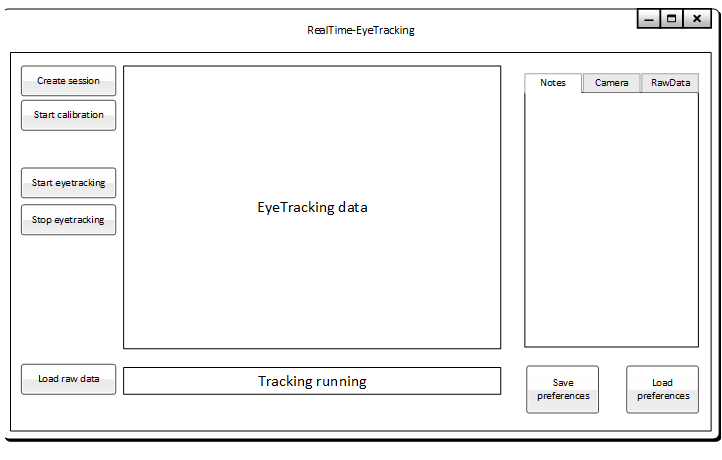
\includegraphics[width=0.7\linewidth]{GUIudkast}
\caption{Udkast til grafisk bruger interface}
\label{fig:GUIudkast}
\end{figure}

\begin{figure}
	\centering
	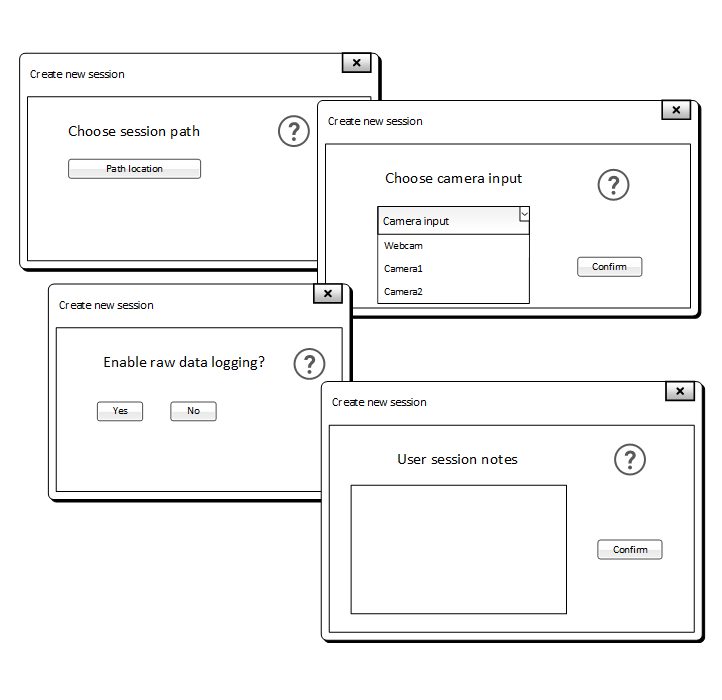
\includegraphics[width=0.7\linewidth]{Undermenuer}
	\caption{Udkast til menuer der guider bruger igennem opsætning}
	\label{fig:Undermenuer}
\end{figure}



\end{document}